\documentclass[crop,tikz]{standalone}
\usetikzlibrary{backgrounds}
\colorlet{blue}{cyan}
\tikzset{
  inverted/.style = {
    color=white,
    background rectangle/.style={fill},
    show background rectangle
  }
}

\usetikzlibrary{calc}
\tikzset{>=latex}
\colorlet{green}{green}

\begin{document}
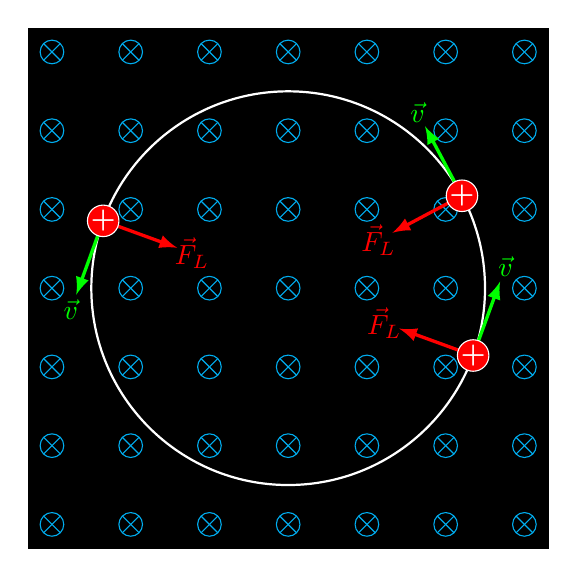
\begin{tikzpicture}[inverted,inverted]
  % magnet field vectors
  \pgfmathsetmacro{\mfrad}{0.15}
  \foreach \X in {-3,...,3} {
    \foreach \Y in {-3,...,3} {
      \draw[blue] (\X,\Y) circle (\mfrad);
      \draw[blue] ($(\X,\Y)+(45:\mfrad)$) -- ($(\X,\Y)+({180+45}:\mfrad)$);
      \draw[blue] ($(\X,\Y)+({90+45}:\mfrad)$) -- ($(\X,\Y)+({-45}:\mfrad)$);
    }
  }
  % circle
  \pgfmathsetmacro{\brad}{2.5}
  \draw[thick] (0,0) circle (\brad);
  % charges
  \pgfmathsetmacro{\crad}{0.2}
  \foreach \angl in {28,160,-20} {
    % velocity
    \draw[->,very thick,green] (\angl:\brad) -- ++({\angl+90}:1);
    \node[green] at ($(\angl:\brad)+({\angl+90}:1.2)$) {$\vec{v}$};
    % Lorentz force
    \draw[->,very thick,red] (\angl:\brad) -- ++({\angl+180}:1);
    \node[red] at ($(\angl:\brad)+({\angl+180}:1.2)$) {$\vec{F}_L$};
    % charge
    \draw[fill=red] (\angl:\brad) circle (\crad);
    \node at (\angl:\brad) {\textbf{+}};
  }
\end{tikzpicture}
\end{document}
